\documentclass[10pt,a4paper]{article}
\usepackage[utf8]{inputenc}
\usepackage{amsmath}
\usepackage{amsfonts}
\usepackage{amssymb}
\usepackage{graphicx}
\usepackage{mathtools}
\usepackage{amsthm}
\author{Pan}
\title{Recent Advances in Studies of Loss Surface of Neural Net}
\newtheorem{pheno}{Phenomenon}
\newtheorem{vp}{Conjecture}
\begin{document}
\maketitle
\section{Context}
A thorough study of the \textit{geometry} or the \textit{landscape} of the loss function of NN(especially deep ones) is a critical step towards a further understanding of \textit{the blackbox}.\cite{open2015} Such a study is also of benefit for the construction of efficient optimization algorithms for deep learning. That is why this topic regains attention in the recent literature of machine learning.

In my latest memo\cite{memo}, I have discussed the possibility of automatically exploiting the one-order geometry of a given loss function for the convenience of applying geometric optimization methods in the context of machine learning. After that, I was aware of the over-generality of my proposed method, which forced me to firstly choose a family of toy loss functions to work with. And this memo is a preliminary context for my future work on my proposed method.   

Actually, the discussion of geometric property of a NN is not a brand new topic. It may be traced back to the introduction of VC-entropy and VC-dimension in statistical learning theory\cite{vapnik2012the} and its application to the study of NN\cite{Anthony2009}. The main idea is to consider the seperating power of a given model on arbitrary distributions. However, these points are too theoretic with a loose relation(at least I have not found out the relation) to what I am studying about. Thus it would not be included in this memo. The ideal style of this memo in my mind should be, as most of the papers I refer to, rich in viewpoints and clear in notations, dealing with some fundamental aspects in machine learning but at the same time, close to problems and phenomena we have met in appplications and experiments.

\section{Outline}
Since this memo is a re-compiled version of half of my paper-based memos over the June, a relatively large number of papers will thus be discussed in this memo. Although the topic is one, \textbf{loss surface of neural net}, both the techniques adopted and the viewpoints are however miscellaneous. An outline may be of help here.

In Section 3, I will discuss the core formulation of \textit{natural gradient descent} introduced by \textit{Amari} in 1998, which is in essence a  \textit{steepest gradient descent} over the parameter manifold equipped with the corresponding \textit{Fisher metric}. The method has been applied to a simple neural net with one hidden layer in the original paper. Although we will no sooner find out that natural gradient descent is general \and theoretically solid but hard to be generalized to deep neural net in a computational efficient way, it is still be considered as a significant breakthrough of geometrical methods applied in NN.

In Section 4, discussion would be concentrated on several specific constraints imposed on the search space that are recently reported\cite{Arjovsky2016} to bring to the learning process more efficiency together with better performance of the same recurrent neural net. The underlying mechanism has not been revealed[ either the imposed \textit{orthogonality} or the \textit{unitarity} seems to come from nothing] and I am extremely curious about it. 

In Section 5, a series of work\cite{Neyshabur201503}\cite{Neyshabur201506} on exploiting the \textit{symmmetry-invariance} in neural net will be discussed. It seemingly lies in the opposite polarity of \textit{natural gradient descent} since it tries to introduce a manifold structure\cite{Badrin2015} via a quite subtle observation of a hiding equivalent relation in the paremter space. The method is at last crystallized into a so-called \textit{$l_p$-path regularizer term}. This paper starts from some experimental observations but comes to a rather general solution, which impresses me a lot.

In Section 6, we finalize this memo by scanning over a series of exciting work that endeavors to depict the loss surface of neural net in a general setting, i.e. arbitrary depth and arbitrary breath. Currently, techniques can be roughly divided to two branches, the first of which is by explicitly studying the analytic property of a NN model or by working out some equivalence with models in physics[\cite{Choro2015} shows its eqivalence with \textit{spin-glass\cite{Stein2004} model} in condensed matter physics. Although it seems like a bootstraping, it whatsoever shows the underlying complexity of how to depict loss surface of NN]. The other branch is experiment-based, depicting the high-dimensional loss surface of a given toy net via some \textit{dimension reduction} methods to some visualizable space or via perturbation around the local minima(or \textit{plateau}) in order to show the local landscape around the plateau. One of these papers will be summarized here\cite{Poggio2017}. Several exciting subsequent work, e.g. answering for what SGD has brought to deep learning\cite{Zhang2017} \and why an slightly over-parameterized neural net will generalize well\cite{Gamst2017}, would also be included. The papers in this section are mostly undergoing researches, inspiring and fascinating me a lot over the whole late June. 

\section{Natural Gradient Descent\cite{Amari1998}\cite{Pascanu2013}}
The discussion of natural gradient can be quite comprehensive if we start from the elements of differential geometry. In fact, natural gradient is a synonym of \textit{gradient} defined on a smooth manifold. It can be referred to in my latest memo\cite{memo}. As a quick review, the main idea here is to generalize the concept of \textit{gradient} in $\mathbb{R}^n$ to arbitraty smooth manifold equipped with some \textit{Riemmanian metric}[A generalized version of inner-product in $\mathbb{R}^n$]. A modifed inner-product induces a quite different language of \textit{'orthogonality'}. That is to say, given a matrix $\mathbf{G}$, we may define the \textbf{G}-orthogonality.
$$
x\perp_{G}{y} \text{ if } \langle{x},y\rangle_{G}\doteq{x}^T\mathbf{G}y=0
$$

As we all know, the steepest gradient descent is based on the orthogonality $\perp$ defined in the search space. With a modifed 'orthogonality' $\perp_{G}$, we may thus apply steepest gradient descent over a geometric structure determined uniquely by the matrices $\mathbf{G}_x$ defined at each point $x$ of the search space. We may list the gradient descent formula as follows[say $\mathit{l}$ the loss parameterized by $w$]
$$
	w_{t+1} = w_{t}-\eta_{t}\mathbf{G}_{w_t}^{-1}\nabla_{w_t}\mathit{l}
$$
, where $(\eta_{t})$ is a monotonicaly decreasing sequence of non-negative scalars.

This roughly reviews the steepest gradient descent over Riemmanian manifold. Now we turn to natural gradient descent, which actually gives several specifications to the general gradient descent.

First, it works with probabilistic models, or a parameterized  distribution family,

$$
	 \mathcal{S} \doteq{\{p_{w}(x):w\in\Theta\}}
$$  

For concreteness, we may formulate a deterministic neural net model into a indeterministic model by injecting some white noise,

$$
\tilde{h} \doteq \sigma(W_{i\to{h}}x)
$$
$$
P_{W}(h|\tilde{h}) \doteq C\exp\{A(h-\tilde{h})^2\}
$$

Since the loss function can be similarly formulated as in the deterministic notation, we will omit it here. How to define a proper Riemmanian metric over the underlying parameter manifold of the distribution family seems more critical.

\textit{Fisher matrix} is a rather old notation from the statistics, while \textit{Amari} lets it revive as a fundamental component in information geometry and thus natural gradient descent.

Say $w\in\mathbb{R}^k$, a proper Riemmanian metric at each point $w$ should thus be in $\mathbb{R}^{k\times{k}}$. In Fisher's notation, it is defined as[again, loss function $\mathit{l}$ parameterized with w] 
$$
	[G_{w}]_{ij} \doteq{\int}\partial_i\mathit{l}\partial_j\mathit{l}p_w(x)\mathbf{d}{x}
$$  
, where $\forall{i,j}\in[k]$, $\partial_{i}l\doteq\frac{\partial{l}}{\partial{w_i}}$

It seems intractable, especially with large-scale problem. We may try to approximate the Fisher matrix at each point with sampling methods since closed form is hard to derive. Despite this bottleneck in practical usage, it was proved to converge in a large convergence rate[that is what the 'efficiency' actually means] with the following updating rule[\cite{Amari1998}, Sec. 4],
$$
	w_{t+1} = w_{t}-\frac{1}{t}\mathbf{G}_{w_t}^{-1}\nabla_{w_t}\mathit{l}
$$

For completeness, we cite a result called '\textit{Cram$\acute{e}$r-Rao Inequality}', which explains what \textit{Amari} means with '\textit{efficient}' in the title of the original paper. 
$$
	\mathbb{E}[(w_t-w^{*})(w_t-w^{*})^{T}]\geq\frac{1}{t}G_{w_t}^{-1}
$$
, where the $w^{*}$ is the global minima.

Although this work has little to do with the following sections, it no doubt at the first time proposed that imposing geometric structure over the search space and appling Riemmanian gradient descent to neural net learning can improve the performance of deep learning. As for me, a side product of this paper is the implicit discovery of the non-trivial local structures of the loss function of neural net. If we could exploit the structures as much as possible, more interesting and efficient learning algorithms would have been constructed. \cite{Pascanu2013} is a good article discussing about some recent methods that can be traced back to natural gradient descent as well.

\section{Several Mysteriously Good Constraints\cite{Arjovsky2016}}
We will discuss about orthogonal constraints $O(n)\doteq\{U\in\mathbb{R}^{n\times{n}}:U^{T}{U}=UU^{T}=\mathbf{I}\}$  on hidden weight of RNN as an example in this section. In the original paper, the unitary constraints $U(n)\doteq\{V\in\mathbb{C}^{n\times{n}}:V^{\dagger}{V}=VV^{\dagger}=\mathbf{I}\}$  has also been proposed in a similar way, omitted for simplicity.

This work is a little specific not because of its constraints but the target optimization problem. Actually, it appears more like a remedy for the explosive or the decaying gradient curse in the RNN structure. By imposing these constraints, it successfully lets the descent step not explicitly scaled by the norm of the weight, which will be formulated in several lines of derivation.

The basic RNN is formulated as,
$$
	z_{t+1} = \mathbf{W}_t{h_t}+\mathbf{V}_t{x_{t+1}}
$$
$$
	h_{t+1} = \sigma(z_{t+1})
$$

Obviously, 
$$
	\frac{\partial{h_{k+1}}}{\partial{h_{k}}} = \mathbf{W}_k^T\mathbf{D}_k
$$
, where $\mathbf{D}_k \doteq{\frac{\partial{\sigma(x)}}{\partial{x}}\bigg{|}_{W_kh_k+V_kx{k+1}}}$



Take C as the loss function, depth $\tau\geq{t}$, then by applying \textit{BPTT}, we may obtain the gradient at timestamp t as[say $h_t\in\mathbb{R}^{d_t}$]
$$
	\frac{\partial{C}}{\partial{h_t}} = (\frac{\partial{h_\tau}}{\partial{h_t}})^{T}\frac{\partial{C}}{\partial{h_\tau}}= (\Pi_{k=t}^{\tau-1}\frac{\partial{h_{k+1}}}{\partial{h_k}})^{T}\frac{\partial{C}}{\partial{h_\tau}}
$$ 

Take the norm at each side,
$$
	\|\frac{\partial{C}}{\partial{h_t}}\| = \|(\Pi_{k=t}^{\tau-1}\frac{\partial{h_{k+1}}}{\partial{h_k}})^{T}\frac{\partial{C}}{\partial{h_\tau}}\|
	\leq\Pi_{k=t}^{\tau-1}(\|\mathbf{W}_k\|\|\mathbf{D}_k\|)\|\frac{\partial{C}}{\partial{h_\tau}}\|
$$
, where the norm is defined as $\|W\| \doteq tr(W^TW)$. Thus with orthogonality contraints, we have
$$
   \|\frac{\partial{C}}{\partial{h_t}}\|\leq(\Pi_{k=t}^{\tau-1}\|\mathbf{D}_k\|)\|\frac{\partial{C}}{\partial{h_\tau}}\|
$$
, which shows the gradient will be bound by something not scaled by weight, thus alleviating the \textit{explosion} phenomenon.

But why I still prefer to call it \textit{mysteriously good}? From my viewpoint, the constaints do not naturally lie in the formalism of either a general neural net or even RNN, at least superficially speaking.[the regularizer in the next section seems more reasonable in this sense]. While its remedy effect on the 'explosion' \and 'decay' is solid as above, I believe it is not the only factor to the considerable improvement of a naive RNN's performance illustrated in figure 1\cite{Arjovsky2016}, with which it works almost as well as a relatively more complicated LSTM. The furtuer study of the loss surface of neural net will be of help to answer this question. In a word, this paper introduces the so-called \textit{unitary evolution recurrent neural net(uRNN)} to alleviate the difficulty in training RNN but unconsciously reveals an unexplainable but interesting experimental phenomenon, which may be of strong relation to the geometric view of the loss surface of RNN in my opinion, a possible direction for furthur research.
\begin{figure}[htb]
      \center{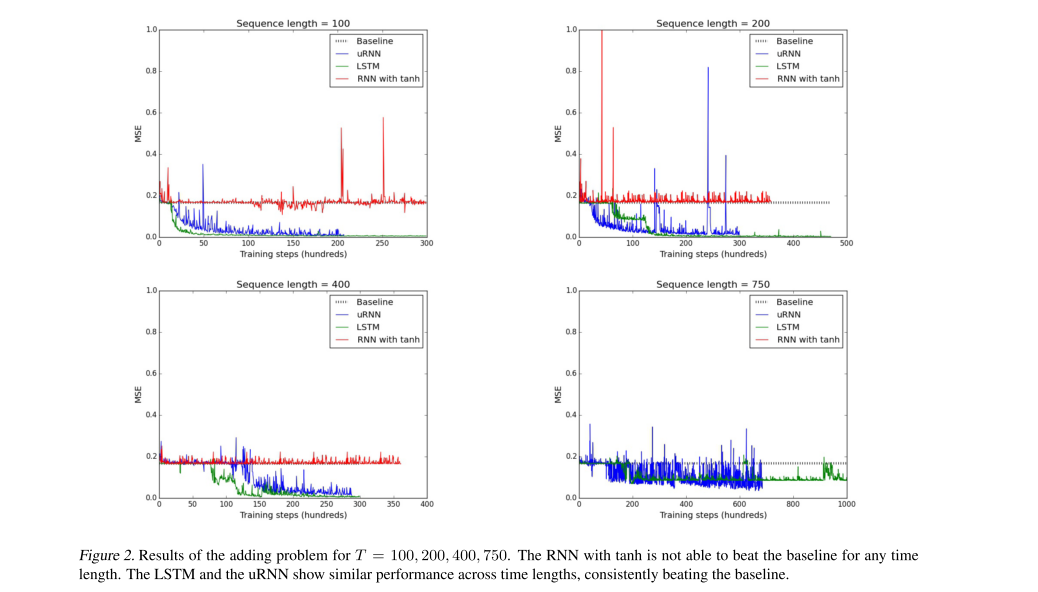
\includegraphics[width=\textwidth]
      {uRnn.png}}
      \caption{\label{fig:my-label} experimental results of unitary evolution recurrent net}
\end{figure}


\section{Exploiting Invariance in NN\cite{Neyshabur201503}\cite{Neyshabur201506}\cite{Badrin2015}}
This series of work begins with an interesting observation in deep neural net with \textit{ReLu} nonlinear layer\cite{Neyshabur201506}. \cite{Neyshabur201506} takes advantage of this observation by introducing a regularizer term from \cite{Neyshabur201503} in loss function, while \cite{Badrin2015} chooses to do the optimization directly on the quotient submanifold induced by the observed equivalent relation. The main idea of the latter is no more than appling gradient descent over a quotient submanifold[details lie in how to derive the projection and retraction operator related with the constructed submanifold] as we have always been discussing about in several latest memos and seminars. Thus in this section, we will rarely talk about  \cite{Badrin2015}.

We first notice such an obvious but non-trivial property of $ReLu$,
$$
	\sigma_{relu}(cx) = c\sigma_{relu}(x) \text{ if }c\geq{0}
$$

Relu becomes popular recently in the architecture extremely deep \textit{CNN} as well as in RNN. And this paper presents that if we adopts \textit{Relu}, we may introduce some extra invariance as well.

Consider the following neurons $x_i^{(n-1)},x_j^{(n)},x_k^{(n+1)}$ with synaptic weight $w_{ij}, w_{jk}$. According to the computational rule of neural net, we have 
$$
	x_k^{(n+1)} = \sigma_{relu}(w_{jk}x_j^{(n)}) =\sigma_{relu}(w_{jk}\sigma_{relu}(w_{ij}x_i^{(n-1)}))
$$

The key observation can be written in the following equality,
$$
	\sigma_{relu}(w_{jk}\sigma_{relu}(w_{ij}x_i^{(n-1)})) = \sigma_{relu}(\frac{w_{jk}}{\lambda}\sigma_{relu}(\lambda{w}_{ij}x_i^{(n-1)})) \text{  } \forall{\lambda>0}
$$

That is to say, by rescaling the weight of the input synaptic weight with $\lambda$ and that of the output synaptic with $\frac{1}{\lambda}$, which immediately induces some equivalent relation over the weight search space.

In graph theory notation, we may formulate a general neural net with \textit{ReLu} nonlinearity as a tuple $(\mathcal{G}=(V,E), w:E\to\mathbb{R})$, where $\mathcal{G}$ is a acyclic graph and weight(or \textit{weight assignment function}) $w$ as a mapping from edges of graph to real line.

With such a notation, we may formulate the invariance in a much clearer style.

Define rescaling transformation of neural net weight as follows,
$$
	\rho_{\lambda,v}(w) \to \tilde{w}
$$

\[
 \tilde{w}(u_1\to{u_2}) = 
  \begin{cases} 
  \lambda{w(u_1\to{u_2})} & \text{if } v=u_1 \\
   \frac{1}{\lambda}{w(u_1\to{u_2})}       & \text{if } v=u_2  \\
   w(u_1\to{u_2}) & \text{otherwise}
  \end{cases}
\]

Thus we denote $\tilde{w}\sim_{\rho}{w}$ if there exists a sequence of transformation $(\rho_{\lambda_{t},v_{t}})$ that transforms $w$ to $\tilde{w}$.

The contributions of this paper did not remain in revealing the above equivalent relation. It however noticed another seemingly independent phenomenon in training a relu NN, that is, 
[\textbf{Note}: 	We call a net is \textit{balanced} if the norm of income weights to different units are roughly the same. Otherwise a net is called unbalanced. See Figure 2\cite{Neyshabur201506}]
\begin{pheno}
	1) Balanced net always generalises better than the unbalanced counterpart.
	
	2) Training will always blow up the small weights but have little effectsw on the large weight.
\end{pheno}

\begin{figure}[htb]
      \center{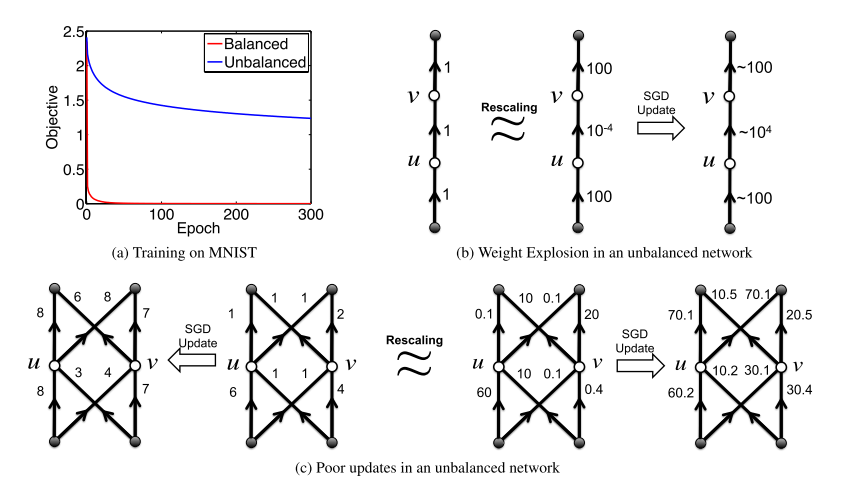
\includegraphics[width=\textwidth]
      {balanced_net.png}}
       \caption{\label{fig:b-label} balanced and unbalanced net}
\end{figure}


Considering this phenomenon, the author proposes to use the group-wise regularization term\cite{Neyshabur201503} with $q=\infty$ to balance the net weight,
$$
	\mu_{p,q}(w) \doteq(\sum_{v\in{V}}(\sum_{(u\to{v})\in{E}}|w_{(u\to{v})}|^{p})^{\frac{q}{p}})^{\frac{1}{q}}
$$

$$
	\mu_{p,\infty}\doteq{sup_{v\in{V}}(\sum_{(u\to{v})\in{E}})|w_{(u\to{v})}|)^{p}}^{\frac{1}{p}}
$$

However, it seems still intractable because of supremum and the hardness of optimizing it over the quotient submanifold induced by $\sim_{\rho}$. The final lemma solves the difficuly totally, which comes from \cite{Neyshabur201503}
$$
	\phi_{p}(w) = min_{\tilde{w}\sim_{\rho}w}(\mu_{p,\infty}(\tilde{w}))^d
$$
where $\phi_{p}$ is called \textit{$l_p$-path regularizer}, defined as follows in a computational plausible way.[which can be computed along the forwarding phase]

$$
	\phi_{p}(w) \doteq (\sum_{i,j}\sum_{v_{in}[i]\to^{e_1}{v_1}\to{v_2}\cdots\to{v_{out}[j]}}|\Pi_{k=1}^{d}w_{(v_{k-1}\to{v_{k})}}|^{p})^{\frac{1}{p}}
$$
, where $v_{in}[i],v_{out}[j]$ are respectively input and output neurons while $d$ the depth. 
  
In summary, this work starts from the observation of \textit{rescaling invariance} in \textit{ReLu} net. It tries to deal with the potential unbalancedness in net training by introduces a quite intuitive $groupwise regularizer$. In order to let the minimization of the regularizer over the quotient submanifold plausible, it constructs the \textit{$l_p$-path regularizer} and proves the equivalence of the two optimization problem.

This work is excellent in its sense for an invariance in NN and also its gentle notations. It does not try to deal with the loss surface problem in a general setting. It comes from a seemingly trivial point but finally comes to something both practical and general(the regularizer). A worth-reading work and the experimental result in Figure 3 shows what more structures to be exploited will in future benefit.

\begin{figure}[htb]
      \center{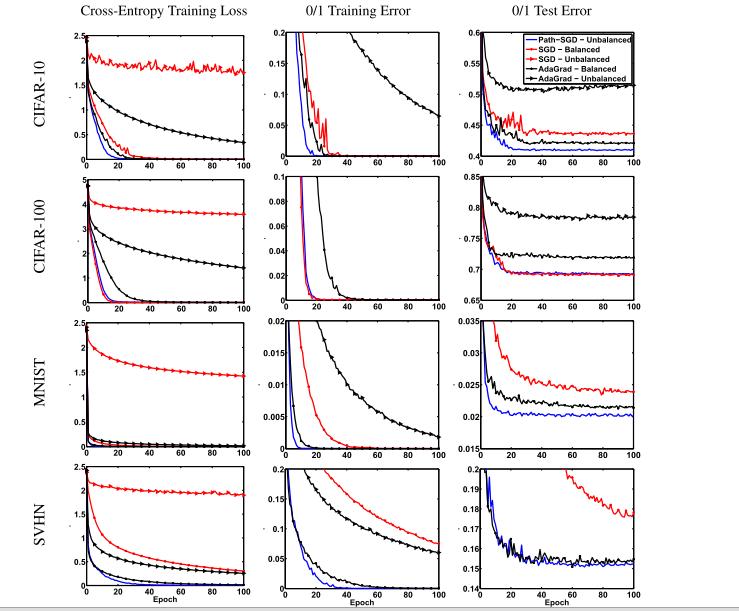
\includegraphics[width=\textwidth]
      {pathsgd_results.png}}
       \caption{\label{fig:c-label} experimental results of path sgd}
\end{figure}


\section{"Scouting" the Loss Surface\cite{Poggio2017}\cite{Zhang2017}\cite{Gamst2017}}
In the final section, I will briefly present some results on the study of loss surface of NN this year. Most of these works are experiment-centered. Although \cite{Poggio2017} has a theoretical part, it is far from convincing. However, as I have written in the outline, I think the research related to this topic would boom in the future since it lies in the core of neural net's mechanism. A better understanding of the loss surface will inspire us to define more sophiscated regularizers, which, as shown in the previous section, would of no doubt be beneficial.

\cite{Poggio2017} presents such a conjecture via a large number of experiments[feel free to refer to the original paper]
\begin{vp}
	We believe that the landscape of empirical risk of an NN is simply a collection of degenerate(degeneracy here means almost all the basins are no better than one another) hyber-basins that each has a flat global minima[see Figure 4]
\end{vp}
\begin{figure}[htb]
      \center{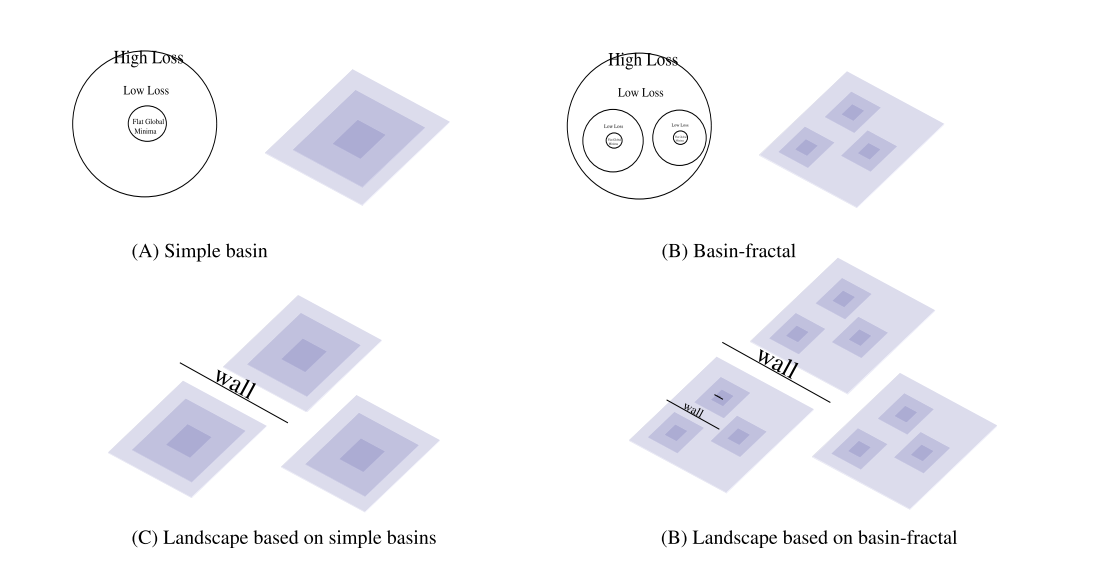
\includegraphics[width=\textwidth]
      {nn_landscape.png}}
       \caption{\label{fig:d-label} a conjecture of the landscape of nn's loss surface}
\end{figure}

\cite{Zhang2017} is a subsequent work of the previous one, which tries to explain why SGD training lets NN generalize well based on the conjectured landscape.

\begin{vp}
	A SGD algorithm(with \textit{lagevin noise}) should asymptotically select among the minimizers the ones that are most degenerate and have a large margin.
\end{vp}
\begin{figure}[htb]
      \center{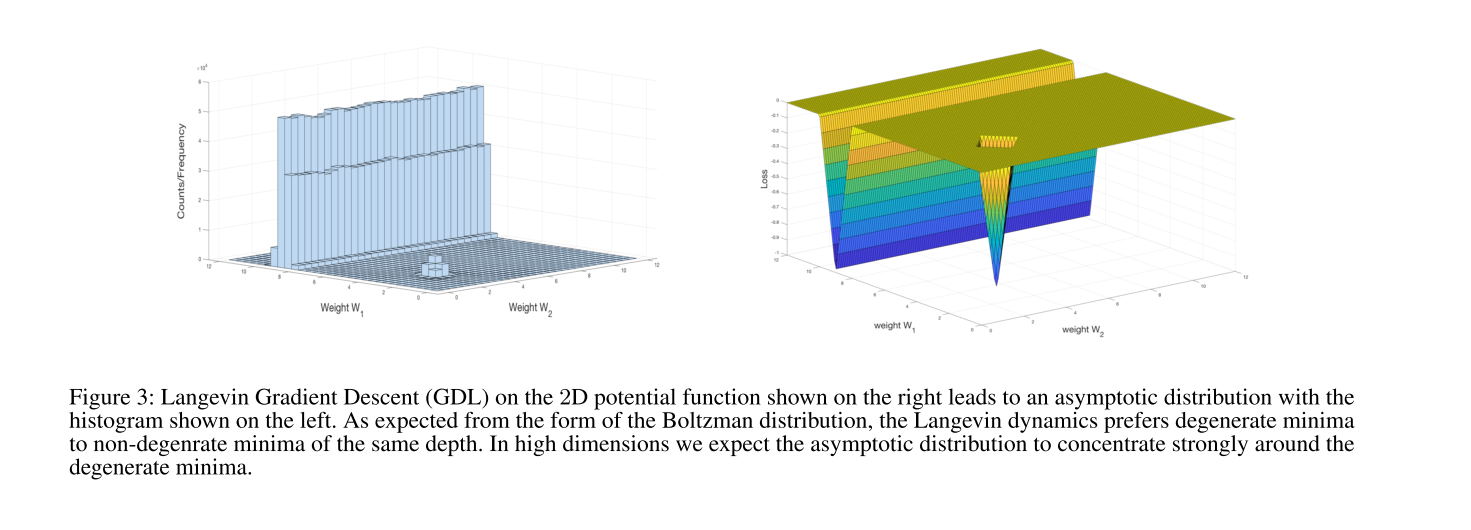
\includegraphics[width=\textwidth]
      {sgd_generalization.png}}
       \caption{\label{fig:e-label} experimental results on the selection of SGDL}
\end{figure}

From the left subfigure in Figure 5, we can see there is a peak and a relatively flat valley on the loss surface, both corresponds to local minimizers. And from the right one in Figure 5, the frequency sgd searches into the flat valley is much larger than it falls into the peak. And in fact, the flatness of a minimizer is directly related with the generalization capability of the minimizer.

The reason of including \cite{Gamst2017} in this memo is that it validates the conjectures of  \cite{Poggio2017}\cite{Zhang2017} from a different starting point. The experiment setting is interesting. It adopts two nets with the same architecture. One works as a teacher net and one learns from the former. The teacher network is manually tuned to generate a signal as in Figure 6\cite{Gamst2017}'s black line.

In such a setting, there is no doubt that the student has the capacity to learn the function represented by the teacher since they have the same structure. However, as shown in Figure 6's red line, the neural net always chooses to filter out the low-frequency signal and discard the high frequency one. In fact, the high frequency ones should always be peaker than the lower ones on the loss surface. That is why I claim it validates the conjectures above. 
 
 \begin{figure}[htb]
      \center{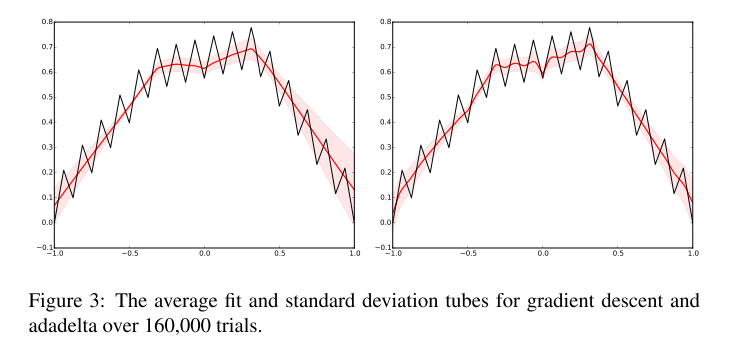
\includegraphics[width=\textwidth]
      {teacher_student.png}}
       \caption{\label{fig:f-label} experimental results on SGD's generalization property}
\end{figure}

As we may notice, the discussion around the loss surface of a general NN is still in its birth phase. Lack of solid theories and full of candidate conjectures while reported phenomena mysterious thus exciting.

I think that is all for this memo on half of my recent readings and thinkings. 


 



\begin{thebibliography}{9}
\bibitem{open2015}Choromanska, Anna, Yann LeCun, and Gérard Ben Arous. \textit{Open problem: The landscape of the loss surfaces of multilayer networks.} Conference on Learning Theory. 2015.
\bibitem{memo} Pan, \textit{Learning Natural Descent via Implicit Approximation of Underlying Parameter Manifold}
\bibitem{vapnik2012the} Vapnik V. \textit{The Nature of Statistical Learning Theory}[J]. Technometrics, 2012, 38(4): 409-409.
\bibitem{Anthony2009}Anthony, Martin, and Peter L. Bartlett. \textit{Neural network learning: Theoretical foundations.} cambridge university press, 2009.
\bibitem{Amari1998}Amari S. \textit{Natural gradient works efficiently in learning}[J]. Neural Computation, 1998, 10(2): 251-276.
\bibitem{Arjovsky2016}Arjovsky, Martin, Amar Shah, and Yoshua Bengio. \textit{Unitary evolution recurrent neural networks.} International Conference on Machine Learning. 2016.
\bibitem{Neyshabur201503}Neyshabur, B., Tomioka, R., \and Srebro, N. (2015). Norm-Based Capacity Control in Neural Networks. Retrieved from http://arxiv.org/abs/1503.00036
\bibitem{Neyshabur201506}Neyshabur, B., Salakhutdinov, R., \and Srebro, N. (2015). Path-SGD: Path-Normalized Optimization in Deep Neural Networks, 1–12. Retrieved from http://arxiv.org/abs/1506.02617
\bibitem{Choro2015}Choromanska, Anna, et al. \textit{The loss surfaces of multilayer networks.} Artificial Intelligence and Statistics. 2015.
\bibitem{Poggio2017}Poggio, Tomaso, and Qianli Liao. "Theory II: Landscape of the Empirical Risk in Deep Learning." arXiv preprint arXiv:1703.09833 (2017).
\bibitem{Zhang2017}Zhang, Chiyuan, et al. Theory of Deep Learning III: Generalization Properties of SGD. Center for Brains, Minds and Machines (CBMM), 2017.
\bibitem{Gamst2017}Gamst, Anthony Collins, and Alden Walker. "The energy landscape of a simple neural network." arXiv preprint arXiv:1706.07101 (2017).
\bibitem{Pascanu2013}Pascanu R, Bengio Y. Revisiting Natural Gradient for Deep Networks[C]., 2013.
\bibitem{Badrin2015}Badrinarayanan, Vijay, Bamdev Mishra, and Roberto Cipolla. "Symmetry-invariant optimization in deep networks." arXiv preprint arXiv:1511.01754 (2015).
\bibitem{Stein2004}Stein, Daniel. "Spin glasses: still complex after all these years?." Decoherence and Entropy in Complex Systems (2004): 147-153.
\end{thebibliography}
\end{document}
